\documentclass{Pretexto/bluereport}

\title{Manual de usuario}
\author{}
\date{}

\begin{document}

\begin{titlepage}
    \thispagestyle{empty}
    
    \pagecolor{white}
    
    % Ahora dibujamos las bandas laterales con \rule{}
    \begin{picture}(0,0)
        % Primera banda (amarilla, la más a la izquierda)
        \put(-94,-800){\textcolor{yellowdark}{\rule{3cm}{99.7cm}}} 
        % Segunda banda (verde)
        \put(-48,-800){\textcolor{yellowlight}{\rule{1.5cm}{99.7cm}}}
        % Tercera banda (azul)
        \put(-20,-800){\textcolor{primaryblue}{\rule{1cm}{99.7cm}}}
    \end{picture}
    
    % Contenido principal de la portada
    \begin{flushleft}
        \vspace*{1cm}

        % Ajusta este valor para mover todo hacia la derecha
        \hspace*{4.5cm}
        \begin{minipage}{13cm} % ancho de bloque de texto
            % Logo 

            
\includegraphics[width=6cm]{img/logo.png}


            \vspace{3cm} 
            
            % Títulos y texto
            {\fontsize{24}{28}\selectfont\color{primaryblue}
            \textbf{COTIZADOR LA LIGA}\par}

            \vspace{2cm}

            {\fontsize{36}{42}\selectfont\color{primaryblue}
            \textbf{Manual de Usuario}\par}
            
            \vspace{1cm}
            
            {\fontsize{16}{20}\selectfont\color{charcoal}
            Versión 1.0\par}
            
            \vfill 
            
            \rule{10cm}{1pt}
            
            \vspace{0.5cm}
            
            {\fontsize{16}{20}\selectfont\color{charcoal}
            Septiembre 2025\par}
        \end{minipage}
    \end{flushleft}
\end{titlepage}


\tableofcontents
\pagebreak

%%%%%%%%%%%%%%%%%%%%%%%%%%%%%%%%%%%%%%%%%%%%%%%%%%%%
\section{Introducción}


%%%%%%%%%%%%%%%%%%%%%%%%%%%%%%%%%%%%%%%%%%%%%%%%%%%%%%%%%%%%%%%%%%%%%%%%%%%%%%%%%%%%
\section{Requisitos del Sistema}

\subsection{Requisitos Mínimos de Hardware}
\begin{center}
\begin{tcolorbox}[
    enhanced,
    boxrule=2pt,
    colframe=primaryblue,
    colback=light,
    rounded corners=5pt,
    width=0.98\textwidth
]

\renewcommand{\arraystretch}{1.6}
\begin{tabular}{>{\raggedright\bfseries}p{3.5cm} 
                >{\raggedright\arraybackslash}p{9.5cm}}

\textcolor{primaryblue}{Procesador:} & 
\begin{minipage}[t]{9cm}
\vspace{-0.3cm}
\begin{itemize}[leftmargin=10pt, itemsep=2pt]
    \item \textcolor{black}{Intel Core i3 de 4ta generación o AMD equivalente}
    \item \textcolor{black}{Arquitectura x64 (64 bits)}
    \item \textcolor{black}{\textbf{Velocidad mínima de 2.0 GHz}}
\end{itemize}
\vspace{0.7cm}
\end{minipage} \\[8pt]
\hline
\textcolor{primaryblue}{Memoria RAM:} & 
\begin{minipage}[t]{9cm}
\vspace{-0.3cm}
\begin{itemize}[leftmargin=10pt, itemsep=2pt]
    \item \textcolor{black}{4 GB de RAM como mínimo}
    \item \textcolor{black}{\textbf{8 GB recomendado para mejor rendimiento}}
    \item \textcolor{black}{Velocidad mínima de 2.0 GHz}
\end{itemize}
\vspace{0.7cm}
\end{minipage} \\[8pt]
\hline
\textcolor{primaryblue}{Almacenamiento:} & 
\begin{minipage}[t]{9cm}
\vspace{-0.3cm}
\begin{itemize}[leftmargin=10pt, itemsep=2pt]
    \item \textcolor{black}{500 MB de espacio libre en disco duro para la instalación base}
    \item \textcolor{black}{200 MB adicionales para base de datos y archivos temporales}
    \item \textcolor{black}{\textbf{Espacio adicional según el volumen de cotizaciones almacenadas}}
\end{itemize}
\vspace{0.7cm}
\end{minipage} \\[8pt]
\hline
\textcolor{primaryblue}{Otros componentes:} & 
\textcolor{black}{\textbf{Conexión a internet recomendada.}} \\[5pt]

\end{tabular}
\end{tcolorbox}
\end{center}

%%%%%%%%%%%%%%%%%%%%%%%%%%%%%%%%%%%%%%%%%%%%%%%%%%%%%%%%%%%%%%%%%%%%%%%%%%%%%%%%%%

\subsection{Requisitos de Software}
\begin{itemize}
    \item Lector de archivos PDF (para visualizar las cotizaciones generadas)
    \item Microsoft Excel o software compatible para crear archivos .xlsx/.xls (opcional, solo si se utilizará la función de importación)
\end{itemize}

\subsection{Sistemas operativos compatibles.}
\begin{itemize}
    \item Windows 10 (versión 1903 o superior)
    \item Windows 11 (todas las versiones)
\end{itemize}

Arquitectura del sistema: x64 (64 bits), no compatible con sistemas operativos de 32 bits.

\subsubsection{Notas adicionales}
\begin{itemize}
    \item La aplicación incluye todas las dependencias necesarias (SQLite, Puppeteer) en el paquete de instalación.
    \item No requiere instalación de Node.js ni otras herramientas de desarrollo.
    \item El archivo de base de datos se almacena localmente y no requiere servidor externo.
\end{itemize}


%%%%%%%%%%%%%%%%%%%%%%%%%%%%%%%%%%%%%%%%%%%%%%%%%%%%
\section{Acceso}
\subsection{Cómo abrir la aplicaión}

Para abir la aplicacion, simplemente haga doble clic en el archivo ejecutable o utilice el acceso directo creado durante la instalación.
%%%%%%%%%%%%%%%%%%%%%%%%%%%%%%%%%%%%%%%%%%%%%%%%%%%%
\section{Interaz Principal y Funcionalidades}
\subsection{Explicación del menú de Gestión de Cotizaciones}

En el menu de getión de cotizaciones, se muestran todas las cotizaciones previamente realizadas, con opciones para editar, eliminar o generar el PDF de cada una.

\begin{figure}[H]
    \centering
    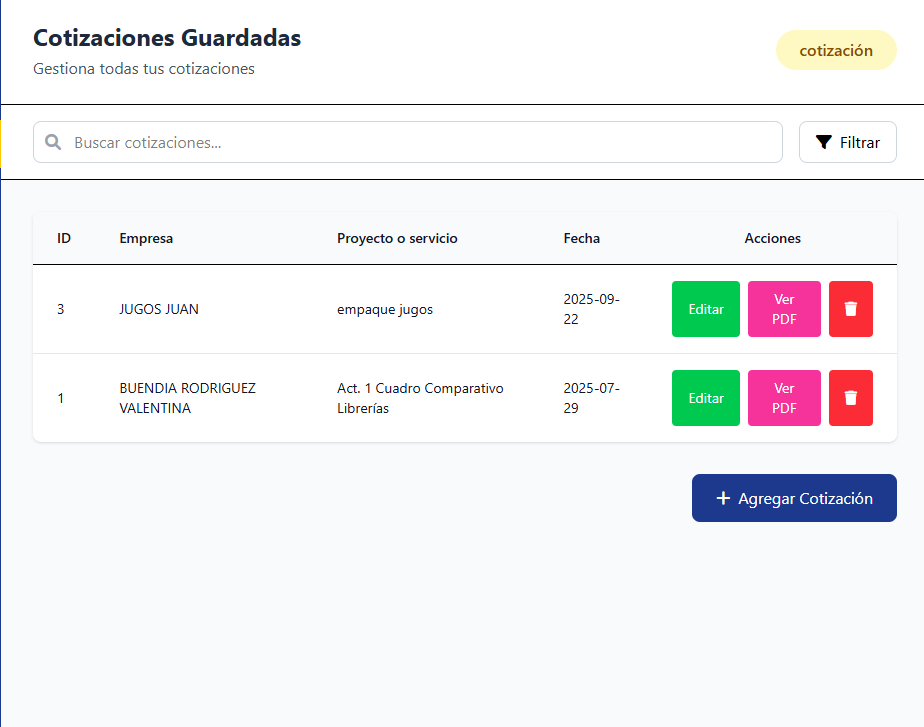
\includegraphics[width=0.8\textwidth]{img/gestion_cotizaciones.png}
    \caption{Menú de Gestión de Cotizaciones}
    \label{fig:gestion_cotizaciones}
\end{figure}

Ademas, se incluye un botón para agregar nuevas cotizaciones.

\begin{figure}[H]
    \centering
    
\includegraphics[width=0.8\textwidth]{img/agregar_cotizacion.png}
    \caption{Botón para Agregar Cotización}
    \label{fig:agregar_cotizacion}
\end{figure}

\subsection{Página para agregar cotizaciones}

En la pagina para agregar cotizaciones, se encuentran varios campos para ingresar los datos necesarios, como el nombre del cliente, la fecha, los productos o servicios a cotizar, y cualquier otro detalle relevante.
Ademas, se incluye un campo para importar datos desde un archivo Excel, para ello, se debe seleccionar el archivo deseado y la hoja correspondiente.

\begin{figure}[H]
    \centering
    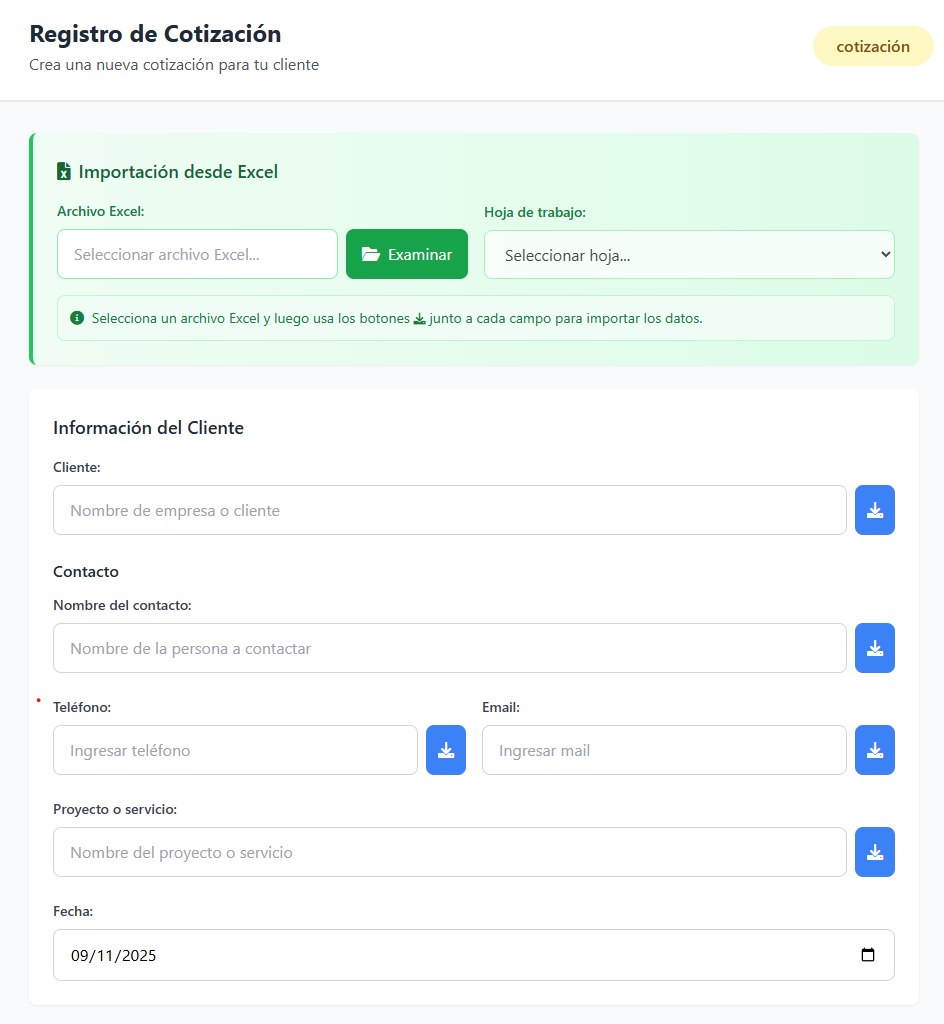
\includegraphics[width=0.8\textwidth]{img/agregar_cotizacion_pagina.png}
    \caption{Página para Agregar Cotizaciones}
    \label{fig:agregar_cotizacion_pagina}
\end{figure}

Para cada campo, hay un boton, que permite al usuario ingresar la informacioón desde el archivo Excel seleccionado, abriendo una nueva ventana con la opcion de dar click sobre la informacion deseada.

\begin{figure}[H]
    \centering
    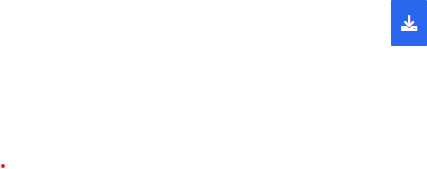
\includegraphics[width=0.8\textwidth]{img/boton_importacion.png}
    \caption{Boton para importar datos desde Excel}
    \label{fig:importar_datos}
\end{figure}

\begin{figure}[H]
    \centering
    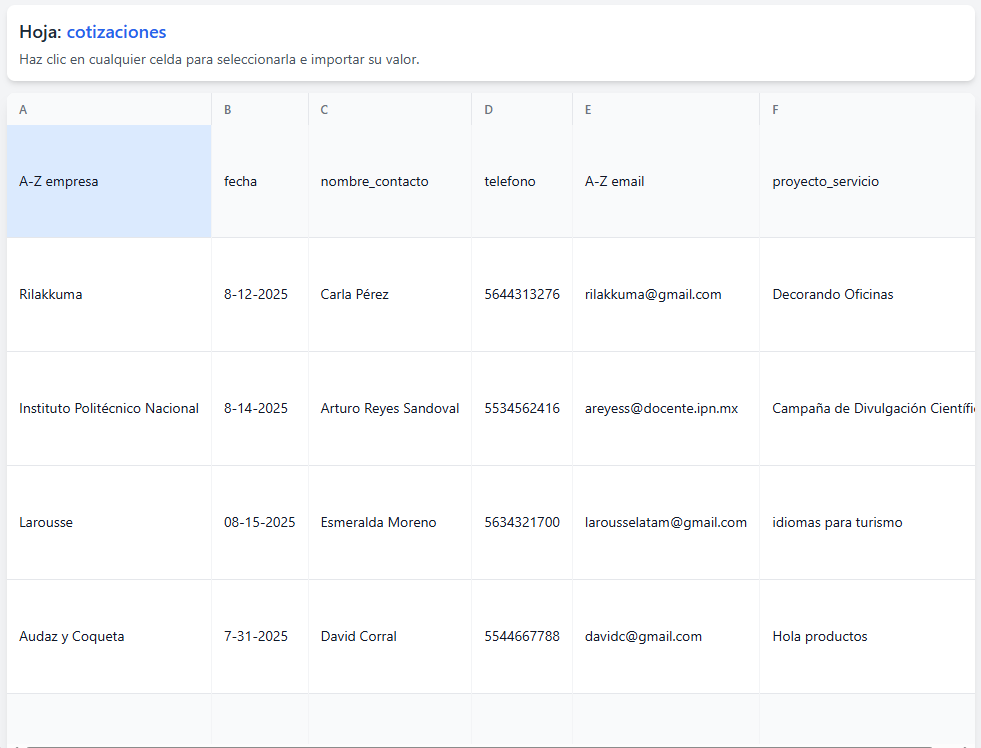
\includegraphics[width=0.8\textwidth]{img/ventana_importacion.png}
    \caption{Ventana de importación de datos}
    \label{fig:ventana_importacion}
\end{figure}


\subsubsection{Gestión de productos/servicios}

Para agregar productos, se incluyo una tabla, donde se pueden agregar, editar o eliminar productos o servicios con campos, con las mismas opciones de importación desde Excel.

\begin{figure}[H]
    \centering
    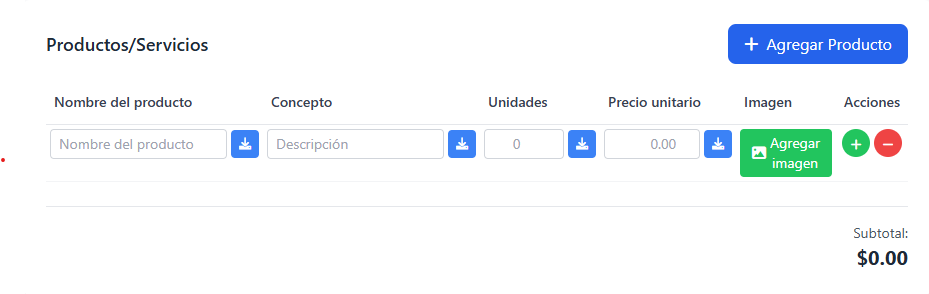
\includegraphics[width=0.8\textwidth]{img/tabla_productos.png}
    \caption{Tabla de productos/servicios}
    \label{fig:tabla_productos} 
\end{figure}

Una vez concluida la cotizacion y verificada la informacion, se puede guardar la cotizacion con el siguiente boton.

\begin{figure}[H]
    \centering
    
\includegraphics[width=0.8\textwidth]{img/boton_guardar.png}
    \caption{Botón para guardar la cotización}
    \label{fig:boton_guardar}
\end{figure}

\subsubsection{Opciones de guardado}

%%%%%%%%%%%%%%%%%%%%%%%%%%%%%%%%%%%%%%%%%%%%%%%%%%%%
\section{Ejemplos prácticos}
\subsection{Cómo registrar una cotización}
Al abrir por primera vez la aplicación, la página de \textbf{Cotizaciones guardadas} se verá como se muestra en la figura 1.
Como aun no hay registros de cotizaciones, la tabla estará vacía. Para agregar una nueva cotización, haz clic en el botón \textbf{Agregar Cotización} o dentro de
la tabla en \textbf{Crear primera cotización}. Esto te llevará a la página para agregar una nueva cotización, donde podrás ingresar los detalles necesarios.
\begin{figure}[H]
    \centering
        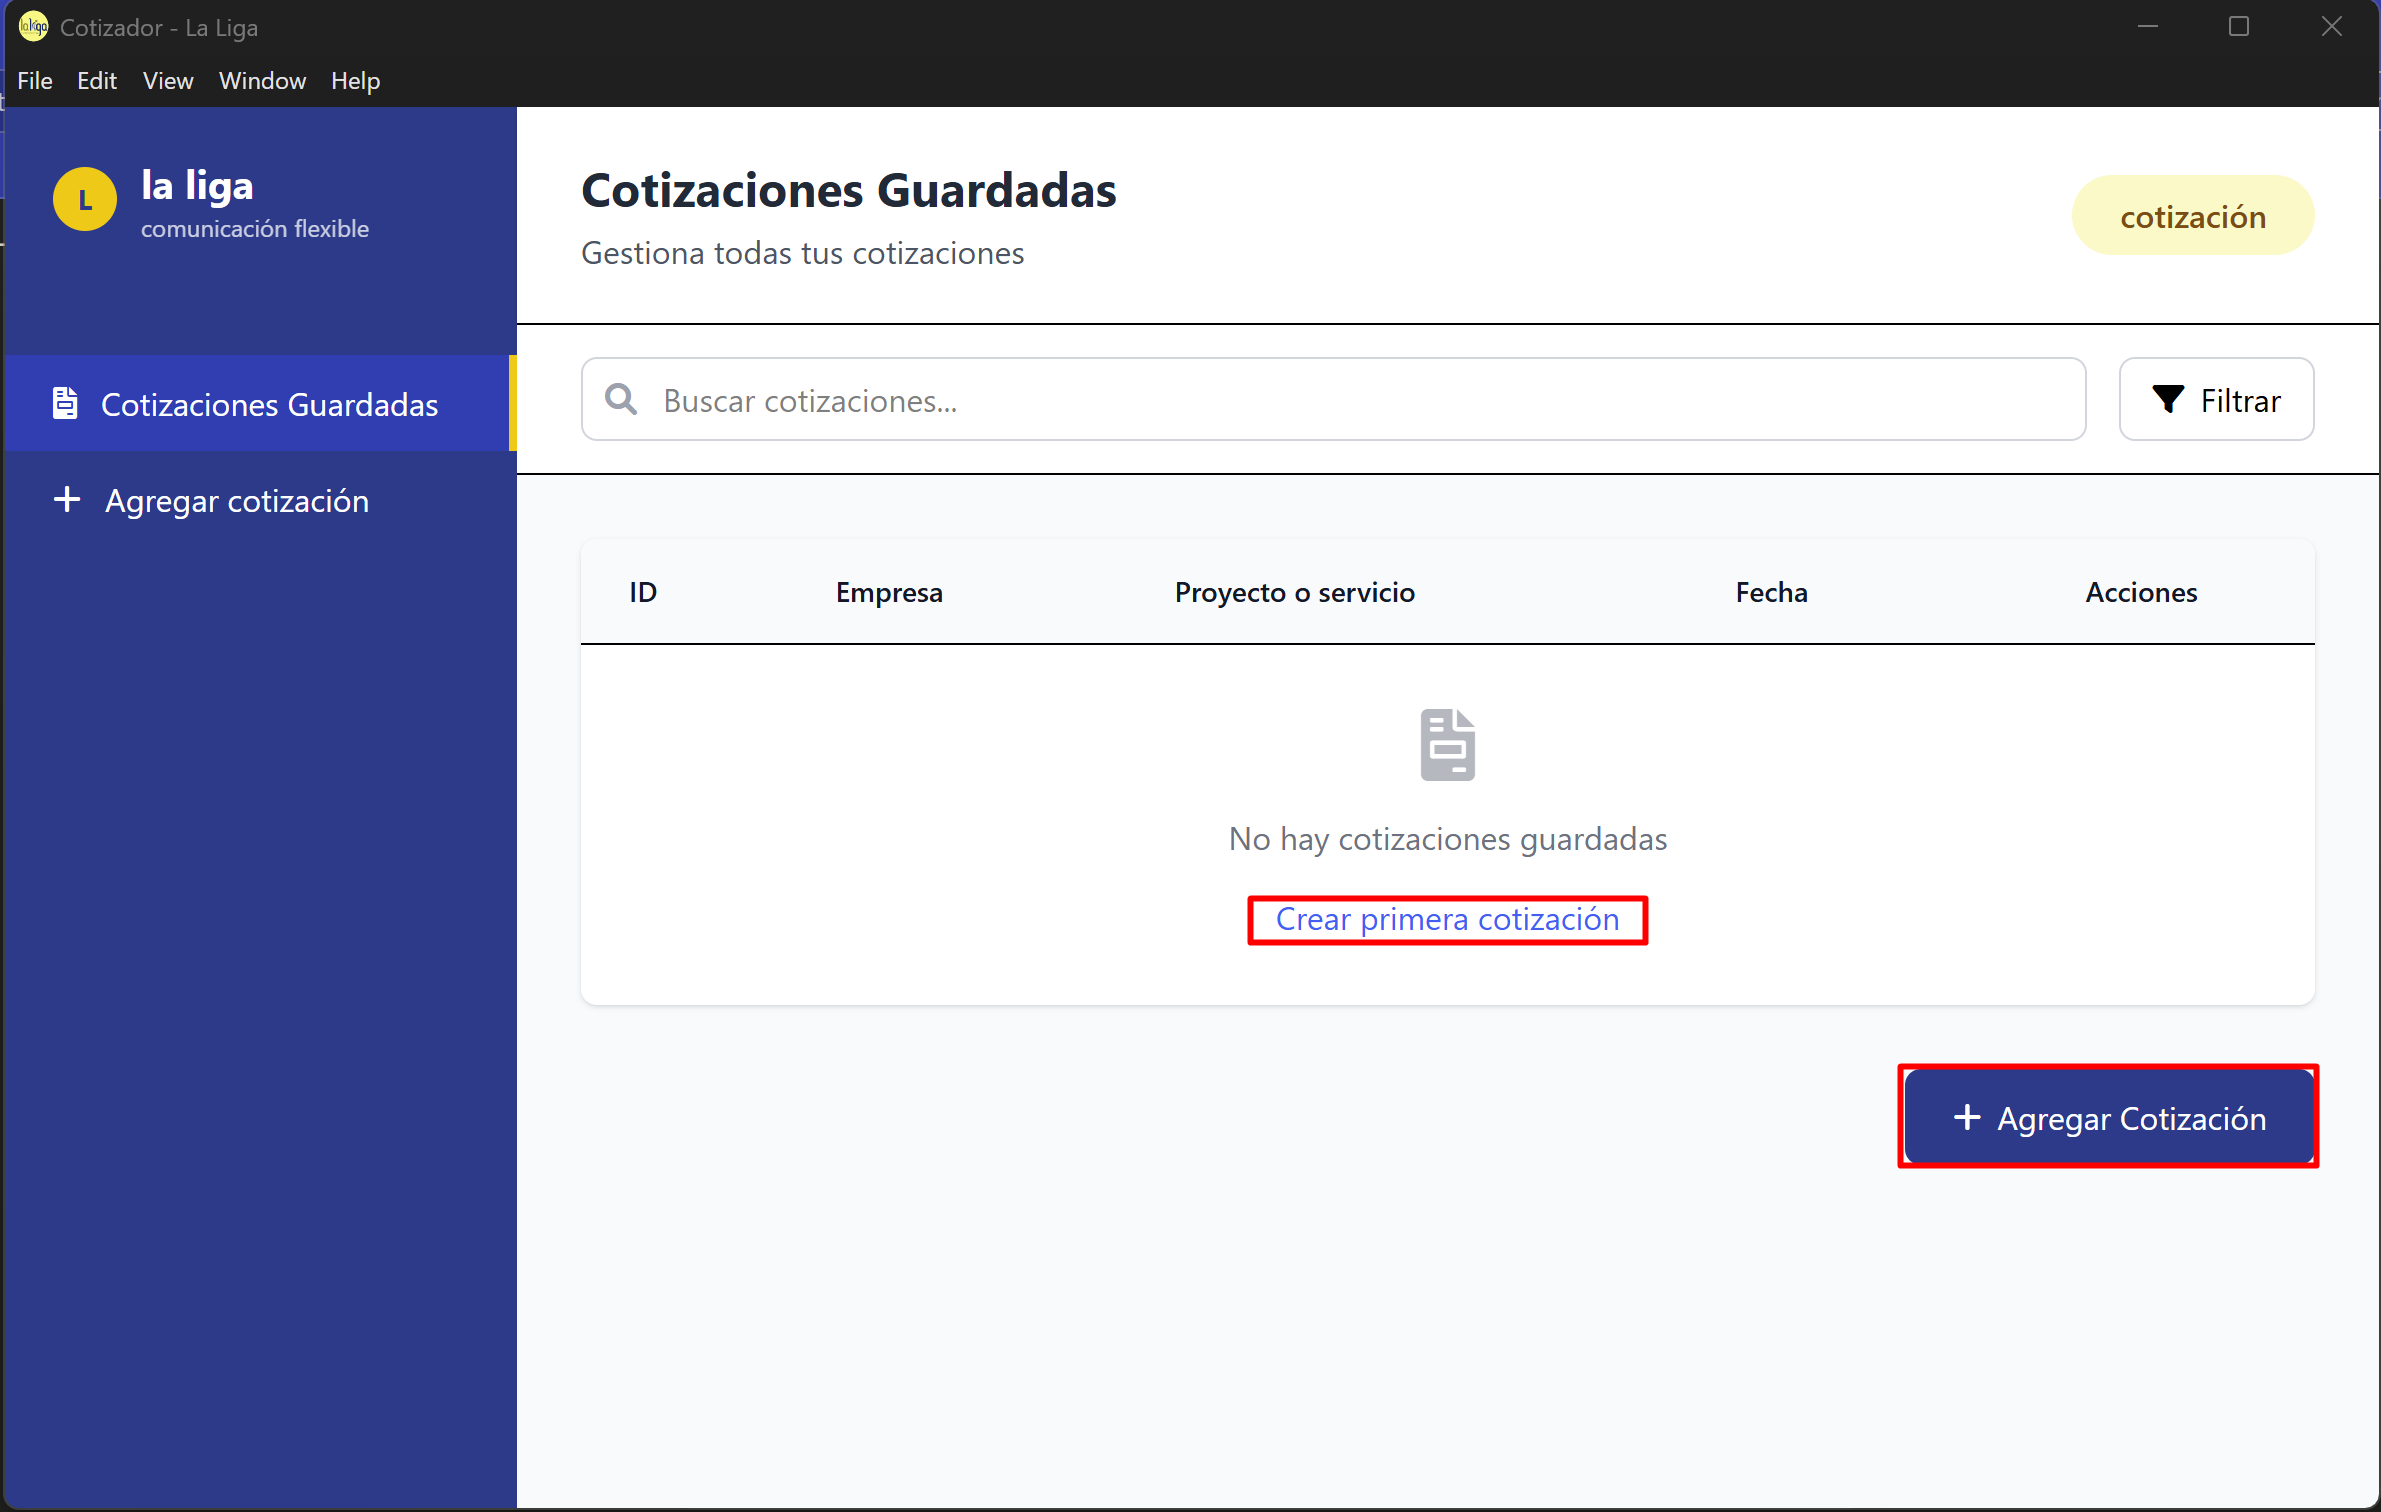
\includegraphics[width=0.85\linewidth]{img/abrir_primera_vez.png}
    \caption{Vista inicial de la página de cotizaciones guardadas al abrir la aplicación por primera vez.}
    \label{fig:vista_inicial}
\end{figure}
Una vez en la página de agregar cotización, podrás ver la siguiente interfaz (figura 2). Aquí podrás ingresar los detalles de la cotización.
\begin{figure}[H] 
    \centering
        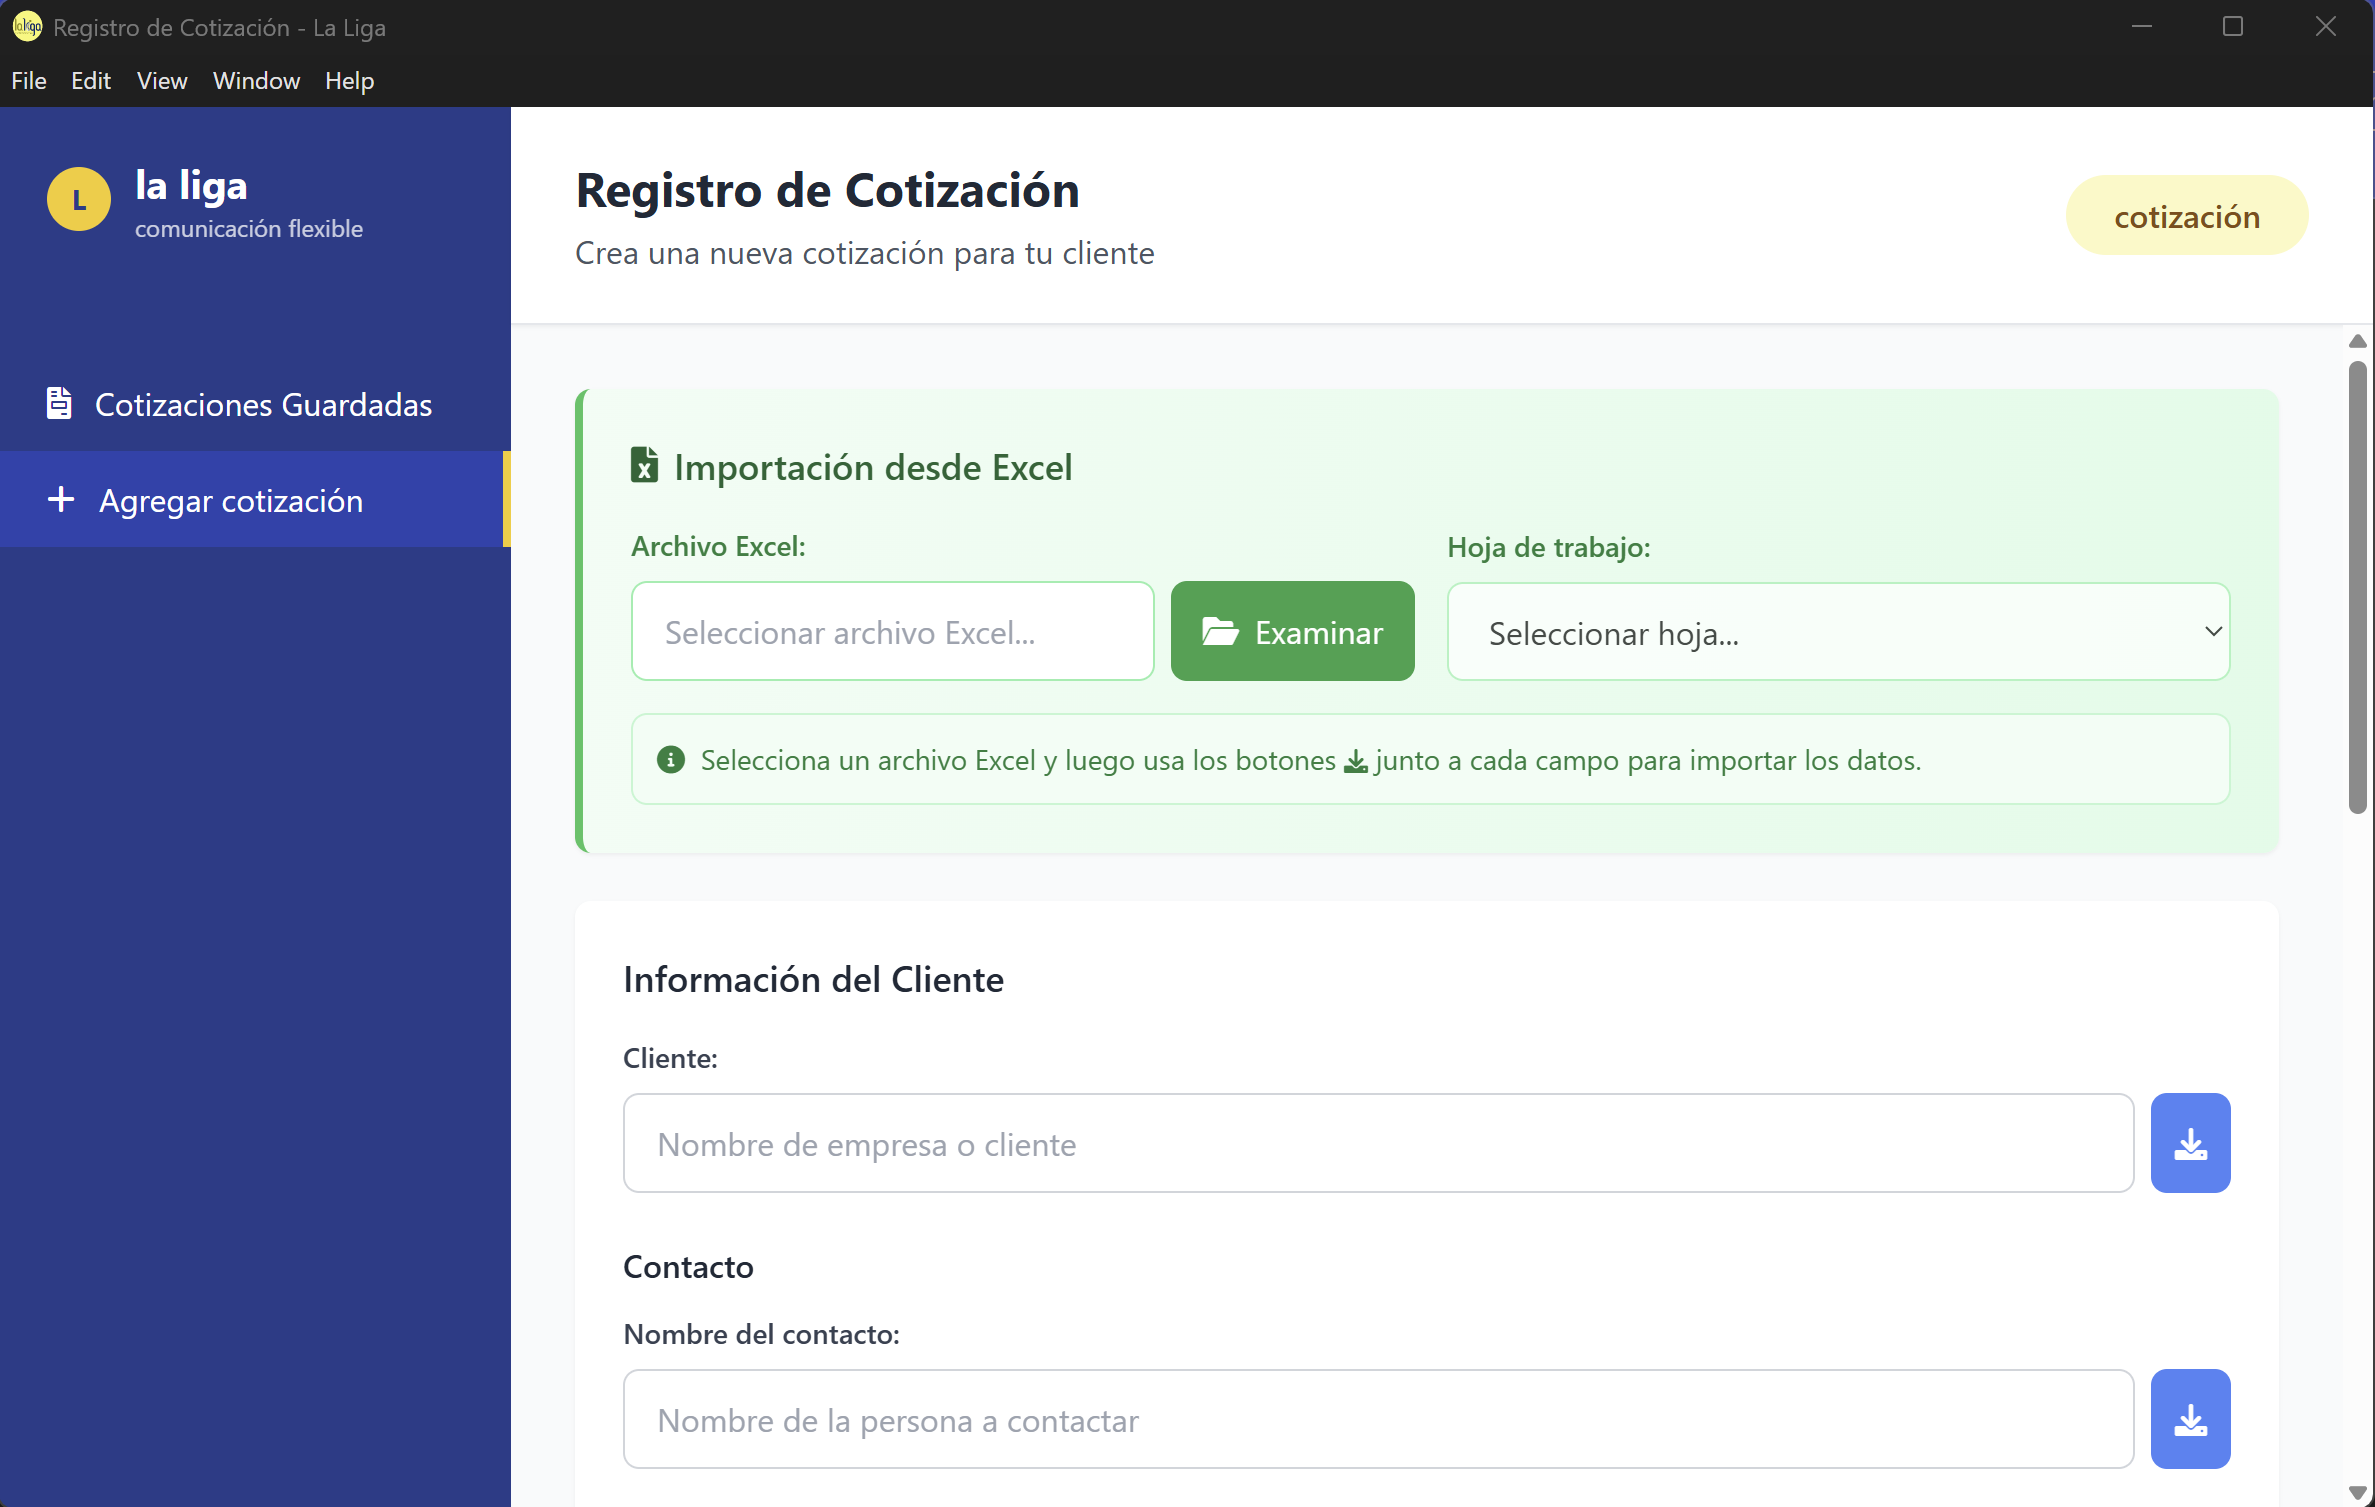
\includegraphics[width=0.85\linewidth]{img/add_cotizacion_inicial.png}
    \caption{Vista inicial de la página de agregar cotización al abrir la aplicación por primera vez.}
    \label{fig:vista_inicial_add}
\end{figure}
En esta parte podrás elegir entre dos opciones para ingresar los datos, la primera es dando clic sobre los campos y escribir a través del teclado.
\begin{figure}[H] 
    \centering
        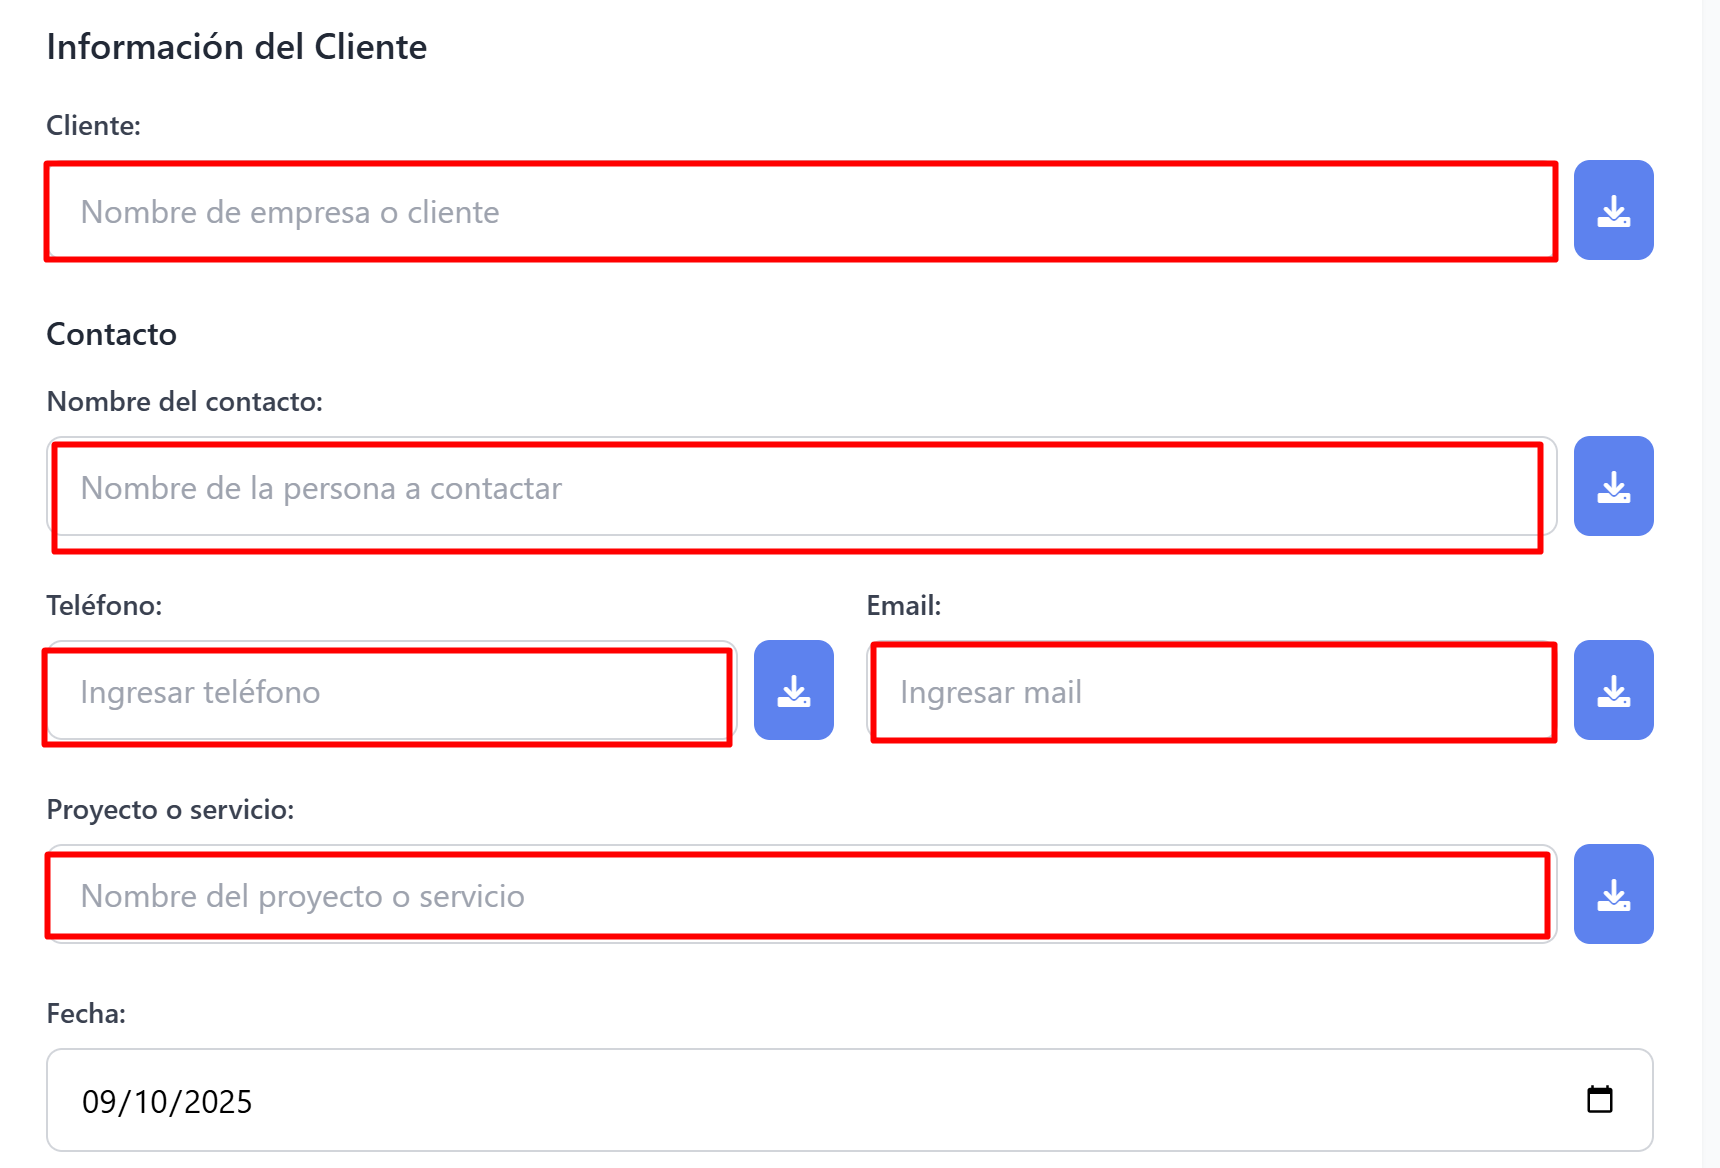
\includegraphics[width=0.85\linewidth]{img/llenar_campos.png}
    \caption{Da clic en los campos y escribe para llenarlos manualmente.}
    \label{fig:llenado_manual}
\end{figure}
La segunda opción es importando los datos desde un archivo de Excel. Para ello, dirígete a la sección de \textbf{Importación desde Excel} que encontrarás hasta arriba de la ventana y haz clic en el botón \textbf{Examinar}. 
A continuación, se abrirá una ventana del Explorador de archivos donde podrás seleccionar el archivo de Excel que contiene los datos de la cotización que deseas importar. Asegúrate de que el archivo esté en formato .xlsx o .xls.

\subsection{Cómo eliminar una cotización}
\subsection{Cómo editar una cotización}
\subsection{Generación del PDF de la cotización}
\subsection{Ejemplo de cotización completa}
%%%%%%%%%%%%%%%%%%%%%%%%%%%%%%%%%%%%%%%%%%%%%%%%%%%%
\section{Resolución a problemas comunes}
\begin{definicion}[No abre correctamente el archivo excel]
    En caso de que no abra correctamente el archivo excel, asegúrese de que el archivo esté en formato .xlsx y que la hoja seleccionada contenga datos válidos. Verifique también que el archivo no esté protegido con contraseña.
\end{definicion}
\vspace{0.7cm}
\begin{definicion}[No se guardan los cambios realizados]
    Este apartado aborda problemas comunes que los usuarios pueden encontrar al utilizar el software, 
    proporcionando soluciones prácticas y consejos para resolverlos.
\end{definicion}
\vspace{0.7cm}
\begin{definicion}[Error al generar el PDF]
    Asegurate de que todos los campos obligatorios esten completos y que haya errores en los datos ingresados. Si el problema persiste, intente reiniciar la aplicación y volver a generar el PDF.

\end{definicion}
\vspace{0.7cm}
\begin{definicion}[No se muestran las imágenes]
    
Asegúrese de que las imágenes estén en el formato correcto (JPEG, PNG) y que la ruta del archivo sea válida. Verifique también que las imágenes no estén dañadas.
\end{definicion}
\vspace{0.7cm}
\begin{definicion}[Problemas al ingresar datos]
    Este puede ser un error comun en la aplicacion, en caso de que no se pueda ingresar algun campo, cambie a otra aplicacion y vuelva a la aplicacion de cotizaciones, esto deberia solucionar el problema.
\end{definicion}



\subsection{Soporte y contacto}

Para aistencia adicional, puedes contactar al soporte técnico a través del correo electrónico: aaronugaldet@gmail.com
\pagebreak

\end{document}